
\documentclass[submit]{ipsj}
%\documentclass{ipsj}

\usepackage[dvipdfmx]{graphicx,xcolor}
\usepackage[T1]{fontenc}
\usepackage{lmodern}
\usepackage{textcomp}
\usepackage{latexsym}
%\bibliographystyle{ipsjunsrt}
\usepackage{subfigure}

%\def\Underline{\setbox0\hbox\bgroup\let\\\endUnderline}
%\def\endUnderline{\vphantom{y}\egroup\smash{\underline{\box0}}\\}
%\def\|{\verb|}

%\setcounter{巻数}{57}
%\setcounter{号数}{1}
%\setcounter{page}{1}


%\受付{2015}{3}{4}
%\再受付{2015}{7}{16}   %省略可能
%\再再受付{2015}{7}{20} %省略可能
%\採録{2015}{8}{1}


\begin{document}


\title{PEGマシンのFPGA実装について}

%\etitle{How to Prepare Your Paper for IPSJ Journal \\
%(ipsj.cls version 2.0)}

\affiliate{YNU}{横浜国立大学}
%IPSJ, Chiyoda, Tokyo 101--0062, Japan}


%\paffiliate{JU}{情報処理大学\\
%Johoshori University}

\author{マイ マイクオン}{Mai Maicuong}{YNU} %[joho.taro@ipsj.or.jp]
\author{本多 峻}{Honda Shun}{YNU}
\author{倉光 君郎}{Kuramitsu Kimio}{YNU} %[gakkai.jiro@ipsj.or.jp]

\begin{abstract}
解析表現文法(PEG)は、2004年にFordによって提案された形式文法であり、
正規表現や文脈自由文法の代替として人気が高まっている。
本稿では、より高い性能要求を目指すため、PEGのFPGA実装、
特にPEG演算子の仮想マシン化によるバーチャルマシン方式について報告し、
性能に関する初期レポートを行う予定である。
\end{abstract}


\begin{jkeyword}
FPGA, PEG
\end{jkeyword}

\maketitle

%1
\section{はじめに}

\cite{latex}

近年、クラウドなどのデータセンターで使うコンピューティングデバイスとして性能向上や電力削減の期待から、FPGAが注目されている。例えば、Microsoft社がWebエンジン「Bing」の処理を高速化するために、自社のデータセンターFPGAを導入すると発表した。また、中国のネット検索サービス大手のBaidu社も画像検索サービスの実装にFPGAの導入を検討している。Intel社でもサーバーCPU「Xeon」のパッケージにFPGAを収める製品を投入する予定である。

一方、データセンターでは、ウイルス対策などのセキュリティ対策が不可欠である。その対策の一つとして、侵入検知システム(IDS:Instruction Detection System)がある。IDSでは、処理は比較的に軽いホスト型IDSが広く使われている。ホスト型IDSは既存の不正アクセスパターンを記憶し、パターンマッチングにより、不正アクセスを検知する。それらのパターンを正規表現で記述することが多い。

FPGA上での正規表現を用いたマッチングマシンに関する研究は様々ある。例えば、研究[]では、実行時間を大幅に短縮することができた。しかし、パターンの複雑度に従い、パターンマッチング回路が非常に大きくなるのは問題である。

本研究では、コンパクト、かつ効率がよいマッチングマシンを実現することを目的としている。そのため、一般的に使われている正規表現の代わりに、解析表現文法(Parsing Expression Grammar)を用いる。PEGはFordによって提案され、正規表現や文脈自由文法の代替として人気が高まっている。PEGの特徴は曖昧性がなく、字句解析が不要であり、また再帰的な構造の処理に向いている。

本研究では、FPGA上でPEGに特化したバーチャルマシンを実現する。必要最小限の回路を搭載し、またPEG演算子に特化した専用回路によってコンパクトかつ効率がよいマッチングマシンを実現する。


%ネットワーク型とホスト型がある。ネットワーク型は、通常の振る舞いとの比較により、不正アクセスを検知するため、処理が重い。一方、ホスト型は既存の不正アクセスパターンを記憶し、パターンマッチングにより、不正アクセスを検知する。そのため、ホスト型の処理は比較的に軽く、現在侵入検知システムとして普及している。
%構文解析とは、定義された文法に従ってテキストの構造を解析することである。この技術はプログラミング言語処理系のみならず、現在Web Page(HTMLやXML)の読み込みやTwitterつぶやきの解析、通信パケットの不正検出など、あらゆる場面で活用されている。現在構文解析を実現するために、正規表現や文脈自由文法という形式文法が広く用いられている。\\

%一方、2004年に解析表現文法(Parsing Expression Grammar)はFordによって提案され、正規表現や文脈自由文法の代替として人気が高まっている(PEG論文)。PEGはPackrat Parsing(PP論文)により線形時間に解析することができる。しかし、Packratは大きな入力に対して莫大なメモリ容量を使用するため、大きなデータの分析に向いていない。そこで、大きな入力を受理するため、MedeirosがPEGのためのVirtual Parsing Machineを提案した(VM論文)。PEGファイルを一つのプログラムに変換して、Virtual Machineで実行される。\\

%一方、近年、IoT(Intenet of things)の発展につれ、様々な機器への組み込みやすさやより高度なパケット処理が必要になった。また、ビックデータ時代になった今は、より高速な構文解析技法が求められている。そのため、組み込みやすさと高速な処理の面から、FPGAが注目されている。構文解析分野でも、FPGAを用いる研究がいくつかある。例えば、文脈自由文法を使ってFPGA上の構文解析\cite{CFG}やFPGA上で正規表現を用いたパターンマッチングマシン\cite{RE1}などの研究がある。\\

%正規表現論文()では、正規表現のマッチングマシンを作るには、3ステップが必要である。まず正規表現を木構造に変換し、次に非決定オートマトンに変換する。非決定オートマトンに変換する際、HDLに変換しやすいように、修正したMcNaughton構造を提案した。最後に非決定オートマトンからHDLに変換する。修正したMcNaughton構造を採用することより、コンパクトな構造が実現できた。一方、文脈自由文法論文()では、文脈自由文法を解析するために、Cocke-Younger-Kasamiアルゴリズムを用いた。\\

%本稿では、より高い性能要求を目指すため、PEGのFPGA実装、特にPEG演算子の仮想マシン化によるバーチャルマシン方式について報告し、性能に関する初期レポートを行う予定である。\\


本稿の構成は次の通りである。第2節はPEGについて述べる。第3節、第4節では、設計及び実装について述べる。第5節に性能評価であり、第6節は結論と今後の課題を述べる。\\


\section{解析表現文法}

PEGはA $\leftarrow$ e というルールの集合であり、その中にAは非終端記号、eは解析表現である。解析表現は表1にある値と演算子を組み合わせた式である。

%+例:

%+正規表現と文脈自由文法と比べる

%\begin{figure}[h]
    %\begin{center}
        %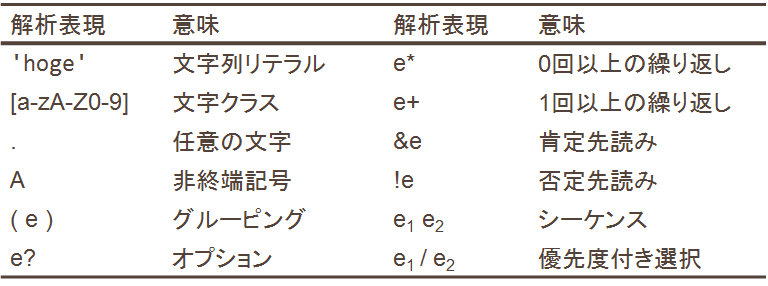
\includegraphics[width=70mm]{./fig/PEG}
       %\caption{PEG}
 %       \label{Ist_list}
    %\end{center}
%\end{figure}

\begin{table}[h]
	\caption{PEGの演算子}
	\centering
\begin{tabular}[t]{lc}
	\hline\hline
	 解析表現 & 意味 \\\hline
	 `hoge' &  文字リテラル \\
	\texttt{[a-zA-Z0-9]} & 文字クラス\\
	 . & 任意の文字 \\
	 A & 非終端記号 \\
	 (e) & グルーピング \\
	 e? & オプション \\
	 e* & 0個以上の繰り返し \\
	 e+ & 1回以上の繰り返し \\
	 \&e & 肯定先読み \\
	 !e & 否定先読み \\
	 $e_1$$e_2$ & シーケンス \\
	 $e_1$/$e_2$ & 優先度付き選択 \\\hline
\end{tabular}
\end{table}

`abc'の場合、入力はabcでないとマッチしないが、[abc]の場合、その中にどれかをマッチすればよい。オペレータ.は任意の文字にマッチする。e?, e*, e+は正規表現と同様であるが、PEGではできるだけ長い文字列をマッチさせる。$e_1$$e_2$は順次に$e_1$、$e_2$を評価し、どちらかが失敗した場合、最初の位置にバックトラックする。優先付き選択($e_1$/$e_2$)はまず$e_1$を評価し、もし失敗した場合$e_2$を評価する。また、!eではeが失敗する時に成功し、eが成功した時に失敗する。

図1は四則演算を表すPEGの例である。

\begin{figure}[h]
    \begin{center}
        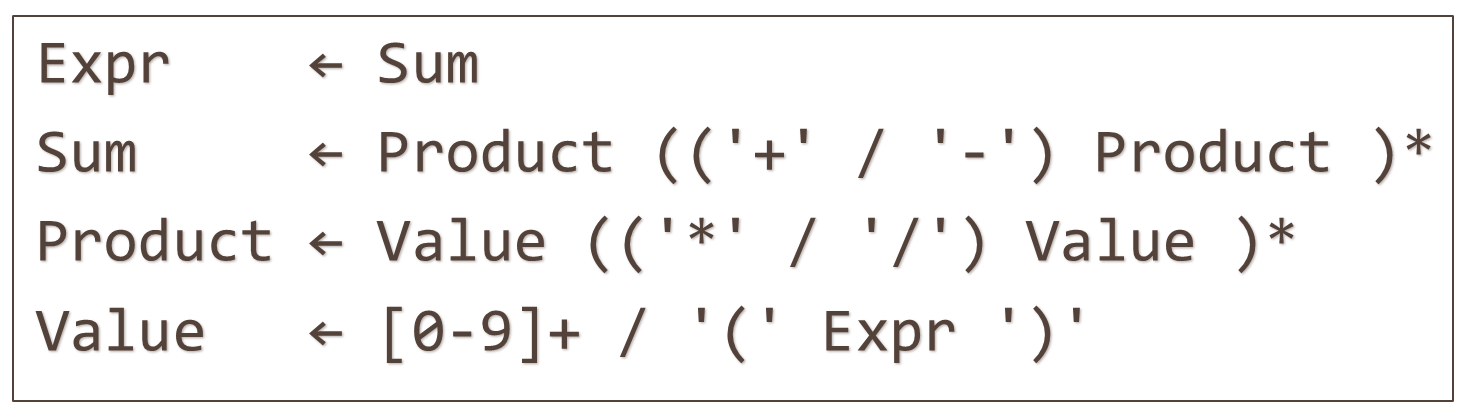
\includegraphics[width=70mm]{./fig/PEG_sample}
       \caption{PEG例}
 %       \label{Ist_list}
    \end{center}
\end{figure}

PEGの演算子が非常に単純で、再帰的構造を処理するのに優れている。また、字句解析及び構文解析を分ける必要がある他の形式文法と違って、PEGでは、字句解析をする必要がない点もメリットとなる。

\section{設計}

PEGはpackrat parsing[]により線形時間に解析することができる。しかし、packrat parsingは大きな入力に対して莫大なメモリ容量を使用するため、大きなデータの分析に向いていない。そのため、大きな入力を受理するため、Medeiros氏がPEGのためのVirtual Parsing Machineを提案した[]。本研究で用いるバーチャルマシンはMedeiros氏が提案したバーチャルマシンをベースにし、命令セットは図2となる。

\begin{figure}[h]
    \begin{center}
        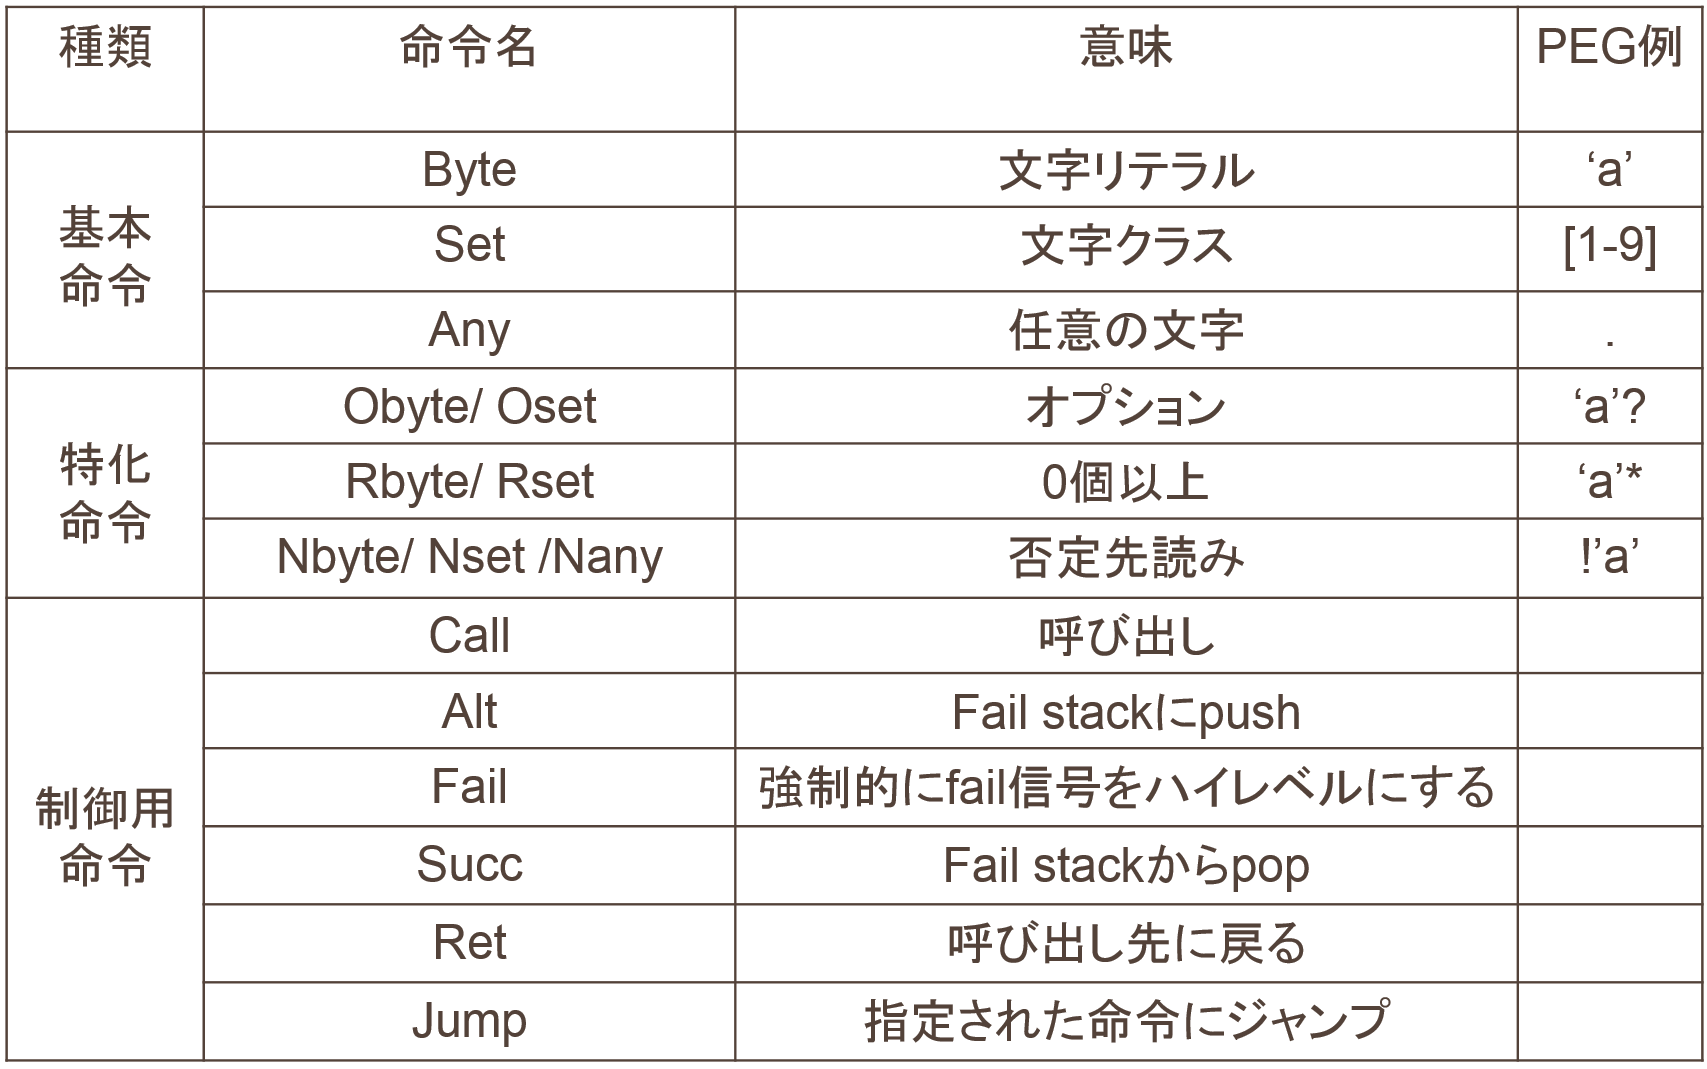
\includegraphics[width=75mm]{./fig/VM1}
       \caption{命令セット}
 %       \label{Ist_list}
    \end{center}
\end{figure}

本研究で用いる命令セットはMedeios氏の提案した命令セットに、PEGの演算子を実行するための特化命令を追加した。特化命令では、オプション命令(Obyte, Oset)、0個以上命令(Rbyte, Rset)及び先読み命令(Nbyte, Nset, Nany)がある。これらの命令は、実行する命令数を削減し、また特化回路によって、実行効率を上げるためである。

メモリ使用量を削減するため、命令のワードは16bitに収めた。第15ビットから第11ビットまでは、オペレーションフィールド(Opフィールド)であり、各命令に対応したコードが割り付けられる。第10ビットから第0ビットまでは命令の対象データとなり、命令によってこのデータの意味が異なる。第10ビットから第0ビットの意味は表2に示すとおりである。

\begin{table}[h]
	\caption{対象データの意味}
	\centering
\begin{tabular}[t]{lc}
	\hline\hline
	 命令 & 対象データの意味 \\\hline
	 Byte/Obyte/Rbyte/Nbyte & 文字 \\
	 Set/Oset/Rset/Nset & Setテーブルのインデックス \\
	 Call/Alt/Jump & 命令アドレス \\\hline
\end{tabular}
\end{table}

%Byte、Obyte、Rbyteの場合、文字である。
%Set、Oset、Rsetの場合、Setテーブルのインデックスとなる。Setテーブルは256行n列の行列であり、8ビットの文字を受け付けて、1ビットを出力する。
%Jump, Call, Alt の場合、命令アドレスを意味する。

%Medeiosが提案したマシンは、次に実行する命令のアドレスを保存するプログラムカウンタ、文字列の現在位置を保存するレジスタ、そしてreturn addressとbacktrack entryを持っているスタックがある。Return addressはプリグラムカウンタのための値である一方、backtrack entryはアドレスと文字列のポジションの両方を持っている。

%基本的な命令は以下となる。\\
%Char x: 文字列の現在位置の文字と文字xをマッチさせ、成功すれば、文字列の位置を1つ増やす\\
%Any: 文字列の末端に到着しなければ、文字列の位置を一つ増やす。文字列の末端に到着すれば、失敗となる。\\
%Choice l : backtrack entryをスタックにプッシュする。lは別の選択肢との相対位置である。\\
%Jump l : 相対位置のlの命令にジャンプする\\
%Call l: 直後の命令アドレスをスタックにプッシュし、相対位置の命令にジャンプする\\
%Return : スタックから一つの命令アドレスをポップし、その命令にジャンプする\\
%Commit l : スタックから一つbacktrack entryを消し、そして相対位置のlの命令にジャンプする\\
%Fail:  スタックからbacktrack entryが出るまでポップし、そのbacktrack entryが新しい状態になる\\

%本研究で採用したバーチャルマシンは上記のバーチャルマシンを拡張したものである。
%扱いやすいために、ReturnスタックとFailスタックに分ける。Returnスタックは、Non-Terminalを呼び出すとき、プログラムレジスタPRの値を退避するためである。Failスタックはバックトラックの戻り値を保存するためである。\\

%MedeiosのVMに以下の命令を追加した。\\
%Set [x-y] : 文字列の現在位置の文字をASCIIの文字でのx以上y以下にマッチさせ、成功すれば、文字列の位置を一つ増やす。\\
 %OChar x, OSet[x-y] :文字リテラル、文字クラスのオプション(以下で述べる)\\ 
%Alt addr: 指定されたアドレスをFail stackにプッシュする\\
%RChar x, RSet[x-y] : 文字リテラル、文字クラスの0個以上\\
%First x addr: 最初の文字がxの場合、addrにジャンプする\\
%NChar x, NSet[x-y], NAny: 先読み\\
%Pos : 文字列の現在位置を専用レジスタに保存する\\
%Back: 保存された位置を文字列の現在位置にする\\

%\subsection{オプション}
%命令数を減らすために、以下の命令を定義する。\\
%OChar x: PEGの'x'?に対応する。文字列の現在位置の文字と文字xをマッチさせ、成功すれば、文字列の位置を1つ増やす。失敗した場合、次の命令に進む。\\
%OSet [x-y]: PEGの[x-y]?に対応する。Setと同様であるが、マッチが失敗した場合、次の命令に進む。\\

%本来であれば、例えば'PEGのx'?は以下の命令列が生成される。\\
%L1 Alt 3\\
%L2 Char x\\
%L3 Commit 1\\

%OChar x を使うことによって命令数を減らすことができた。

%\subsection{0個以上と先読み}
%同様に、以下の命令を定義する。\\
%RChar x : PEGの'x'* に対応する。文字列の現在位置の文字と文字xをマッチさせ、成功すれば、文字列の位置を1つ増やし、もう一回実行する。マッチされなくなれば、次の命令に進む。\\
%RSet [x-y] : PEGの[x-y]*に対応する。文字列の現在位置の文字をASCIIの文字でのx以上y以下にマッチさせ、成功すれば、文字列の位置を一つ増やし、もう一回実行する。マッチされなくなれば、次の命令に進む。\\
%NChar x: PEGの!'x'に対応する。Char xの逆であり、マッチされれば、失敗となる。マッチされなければ、成功となり、次の命令に進む。ただし、文字列の位置を変更しない。\\
%NSet [x-y] , NAny: それぞれPEGの![x-y]に対応する。NChar x と同様である。\\


\section{実装}

\subsection{全体図}

全体のシステムは図3に示すとおりである。ホストとの通信はUbuntu OSとFPGAの通信が可能にした、Xillybus社が提供しているXillybus IPコアを用いる。また、メインメモリはFPGAに搭載しているブロックメモリで実装する。システムの動作では、まずホストから命令列のバイトコードを受け取り、メモリに一時的に保存する。次に文字列をホストから受け取り、解析を行い、結果をホストを返す。

\begin{figure}[h]
    \begin{center}
        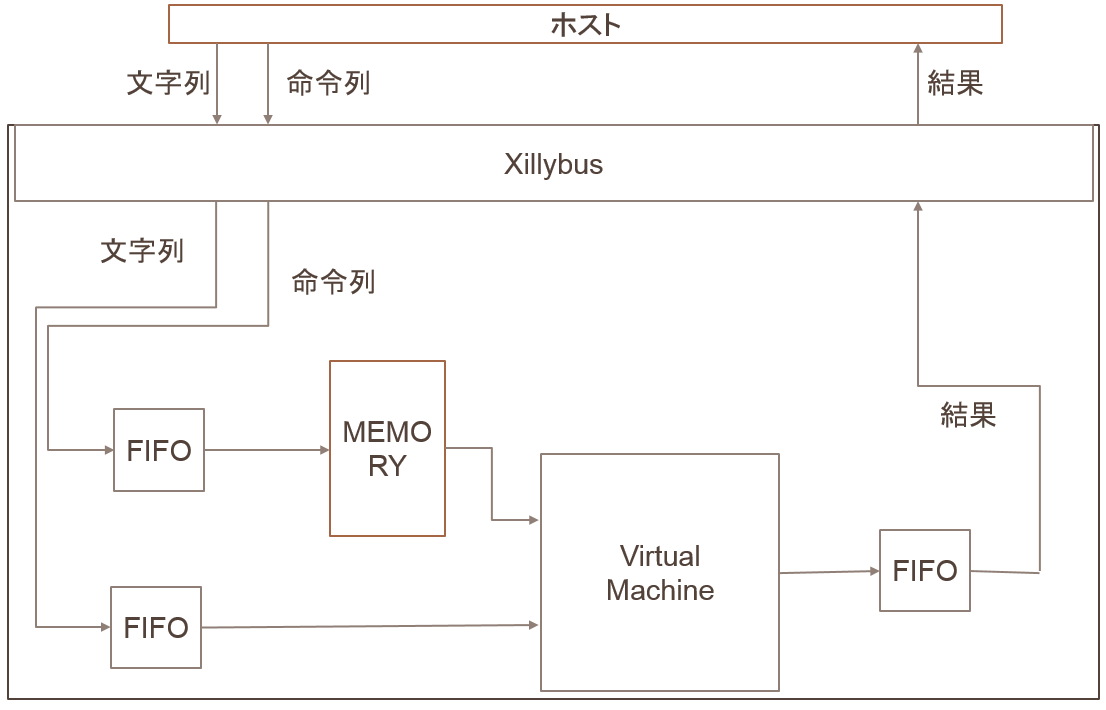
\includegraphics[width=70mm]{./fig/system}
      \caption{全体システム}
 %      \label{Ist_list}
    \end{center}
\end{figure}

また、PEGに特化したVirtual Machine(PEGVM)の全体図は図4となる。PEGVMには、書き換え機能つきプログラムレジスタ(PR)がある。PRは次に実行すべき命令が格納されたメモリアドレスを指定する。プログムの実行に従って順次にインクリメントされ、ただし、分岐命令や割り込みが実行された場合、分岐先のアドレスがPRに書き込まれる。

また、ReturnスタックとFailスタックがあり、それぞれのスタックがスタックポインタを持っている。スタックポインタは、インクリメンタとディクリメンタを持っており、信号によってインクリメントやディクリメントが適時実行される。

他に、命令を解読するデコーダやそれぞれの命令に特化した命令用回路がある。また、メモリから読み込んだ命令データ、FIFOから受け取った文字データはそれぞれ命令レジスタ(IR)、文字レジスタ(TR)に一時的に保存される。

\begin{figure}[h]
    \begin{center}
        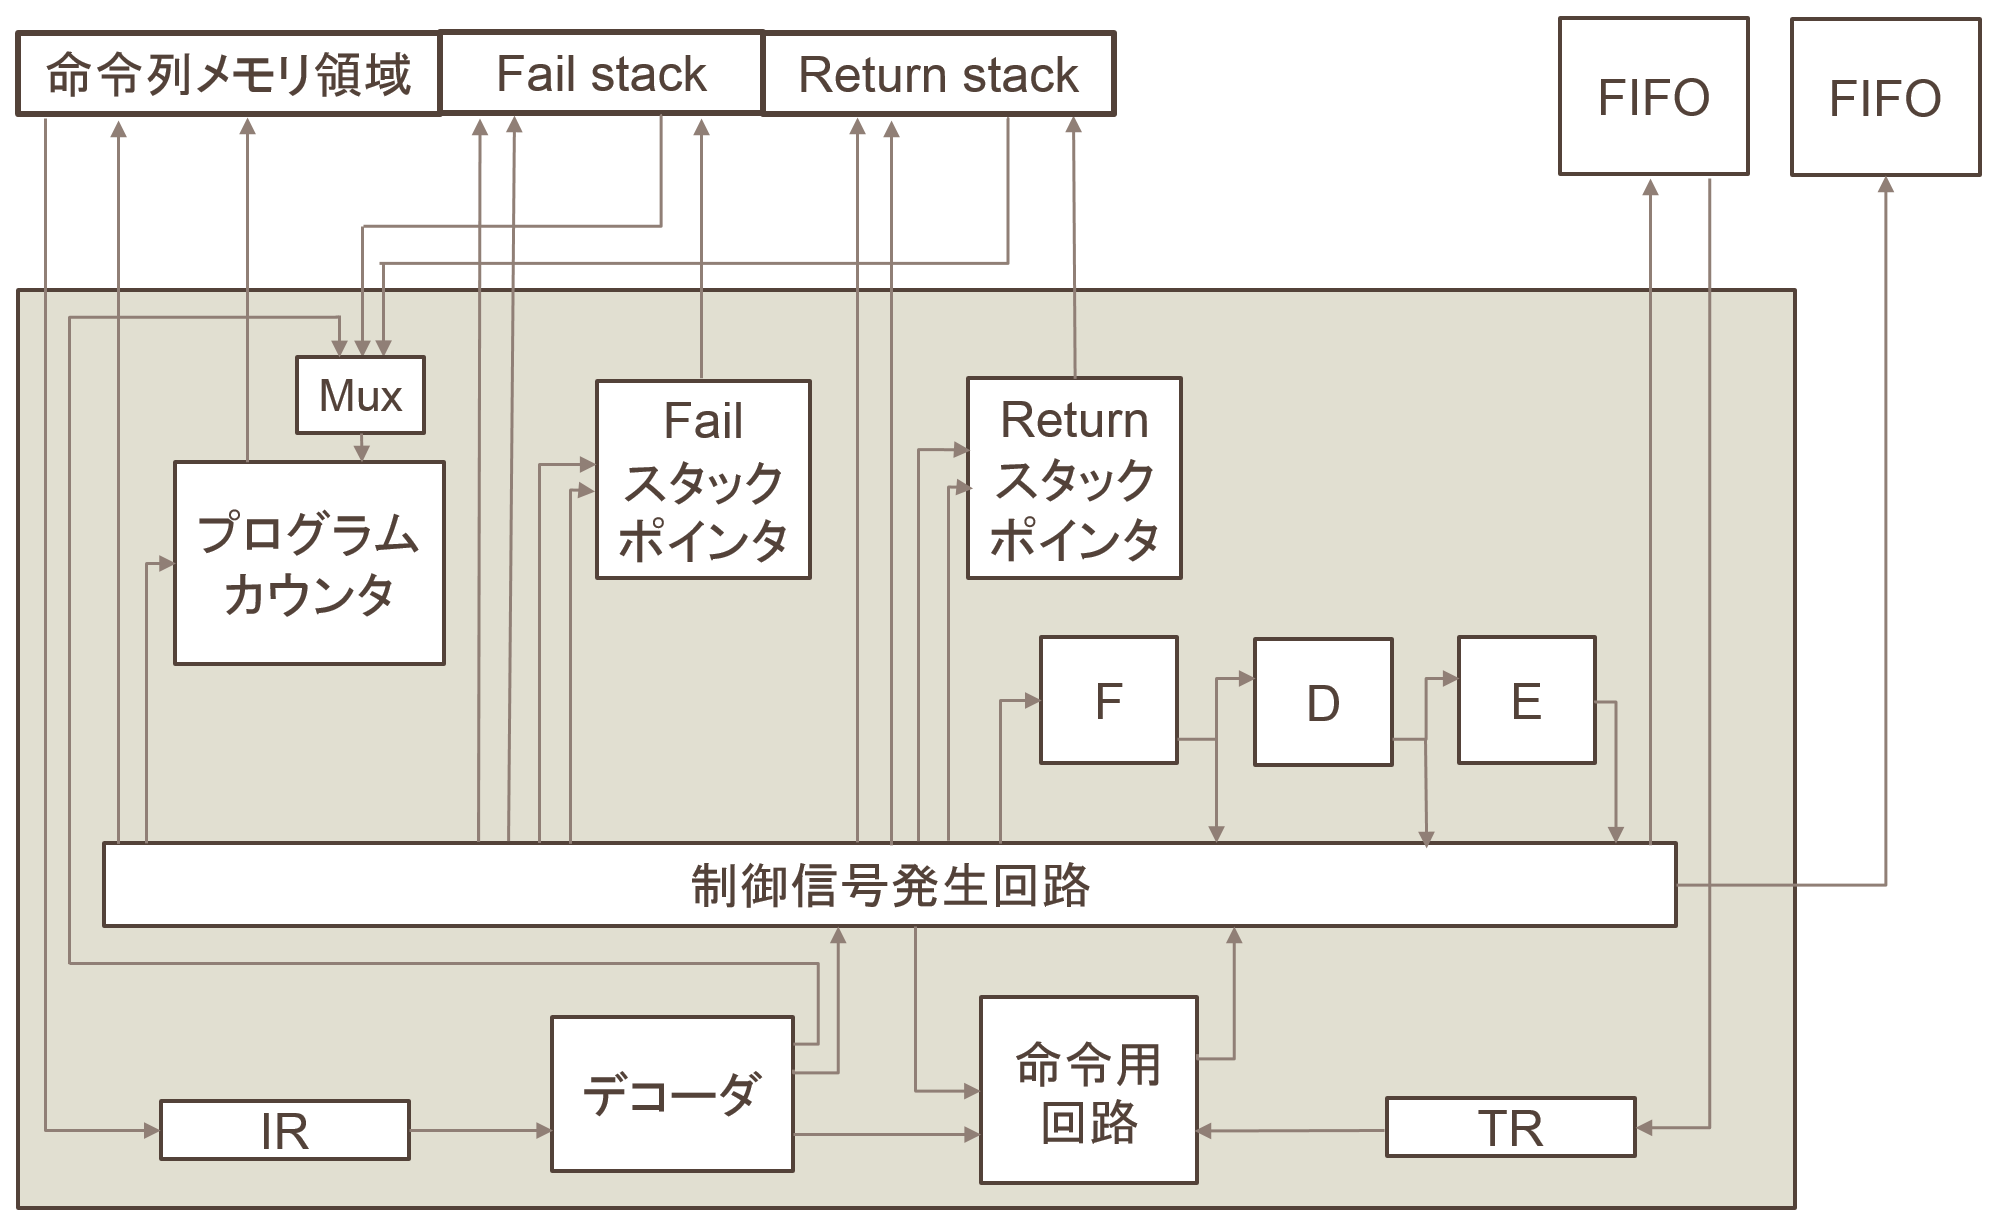
\includegraphics[width=70mm]{./fig/circuit}
       \caption{Virtual Machineの全体図 }
 %       \label{Ist_list}
    \end{center}
\end{figure}

\subsection{PEGVMの動作}

PEGVMの動作は、命令フェッチ、文字データ読み込み、命令デコード、及び演算・データ転送を行う命令実行といった一連の処理の繰り返しであり、それらに対応したF、D、Eという3つの状態がある。一般的に、命令フェッチは命令が格納されているメモリアドレスの設定、メモリデータレジスタへの読み込み、命令レジスタへの転送の3つの動作で構成される。しかし、本実装ではFPGAに搭載しているBlockRAMをメモリとして使用するため、命令フェッチは1クロックサイクルで実行できた。実際に、メモリアドレスは事前に設定しておき、読み出し信号がある場合、データをメモリデータレジスタを通さず、直接命令レジスタに転送される。D状態も1クロックサイクルで実行される。E状態は基本的に1クロックサイクルで実行されるが、Rbyte、Rsetや分岐命令の場合は例外であり、具体的に4.3節で説明する。

制御信号生成回路の役割は、制御信号を適時生成して、各回路に伝えることである。状態F、D、Eに対して、3つのフリップフロップが直列に接続されている。まず前の命令の実行が成功した場合、状態Fに対するフリップフロップにフェッチ起動信号のハイレベル値が取り込まれる。そのクロックの間、メモリへの読み出し信号がハイレベルにする。

その次のクロックの立ち上がりで、状態Dに対するフリップフロップにハイレベルが取り込まれ、状態Fに対するフリップフロップの出力値はローレベルになる。そのクロックの間、IRが持っている命令データがデコードされる。同様にして、その次のクロックサイクルでは、命令実行のための信号がハイレベルにして、命令を実行する。そして、次のクロックから新たな命令フェッチを実行する。


%\subsubsection{ハードウェア仕様}
%NezProcessorのワードは16ビットである。


%\subsubsection{命令の形式}
%第15ビットから第11ビットまではオペレーションフィールド(Opフィールド)であり、各命令に対応したコードが割り付けられる。第10ビットから第0ビットまでは命令の対象データとなる。命令によってこのデータの意味が異なる。
%Byte、Obyte、Rbyteの場合、文字である。
%Set、Oset、Rsetの場合、Setテーブルのインデックスとなる。Setテーブルは256行n列の行列であり、8ビットの文字を受け付けて、1ビットを出力する。
%Jump, Call, Alt の場合、命令アドレスを意味する。


%制御部はそのための制御信号生成回路と、命令を解読するためのデコーダから構成される。\\
%命令フェッチは命令が格納されているメモリアドレスの設定、メモリデータレジスタへの読み込み、命令レジスタへの転送の3つの動作で構成される。命令デコードでは、命令レジスタに取り込まれた命令のビットパターンから、どのような演算・データ転送を行うかを判断する。


%\subsubsection{命令フェッチ}
%NezProcessorでは、FPGAに搭載したBlockRAMをメインメモリとして、使う。FPGAでは、メモリを作るには、FFRAM、LUTRAM及びBlockRAMという3つの方法がある。大容量のメモリが必要な場合、BlockRAMはよく使われている。論理合成する際、メモリへの書き込み・書き出しが同期・非同期かによって、どのメモリを使うか、合成ツールが推論する。BlockRAMに推論されるために、書き込み・読み出しが同期でなければならない。
%前の命令でのEx状態で、次の命令アドレスの設定を行う。そして、F1状態でメモリにアクセスし、IRに転送する。Dec状態では、IRのデータをデコードする。この処理が繰り返される。
%\subsubsection{デコードと演算・データ転送}

%\subsubsection{制御信号生成回路の構成}
%NezProcessorの制御信号生成回路は、配線論理制御方式を採用している。配線論理制御方式は、目的の状態遷移をもつ順序回路によって制御を行う。図()に制御信号生成回路を示す。状態F1,Dec、Exに対して、3つのフリップフロップが直列に接続されている。

\subsection{各命令の実行}

\subsubsection{基本命令}

Byte命令実行のタイムチャートは図5aに示す。F状態では、クロックの立ち上がりで命令読み込み信号のread\_ist信号がハイレベルになり、命令が格納されるメモリにアクセスし、データを命令レジスタ(IR)に転送される。アクセスアドレスはプログラムレジスタ(PR)から転送されたアドレスである。同時に文字読み込み信号read\_text信号もハイレベルになり、FIFOから1文字を読み出し、文字レジスタ(TR)に転送される。

次のクロックの立ち上がりで、IRとTRのデータが確立され、このクロックサイクルでIRのデータがデコードされ、どの命令を実行するかが決まる。今回はByte命令用回路が実行されることになる。同クロックサイクルで、PRはインクリメントされ、メモリアクセス用のレジスタのaddrにデータが転送される。

次のクロックサイクルの立ち上がりで、Byte命令用回路のトリガーであるByte\_rがハイレベルになり、Byte命令用回路が実行される。IRが持っている文字データとTRの文字データが一致するならば、match信号がハイレベルになり、一致しなければ、fail信号がハイレベルになる。match信号及びfail信号は、制御信号生成回路の入力であり、match信号がハイレベルであれば、次のクロックから新たな命令フェッチを実行するように制御信号が生成される。一方、fail信号がハイレベルの場合、Fail処理を実行する制御信号が生成される。Fail処理では、Failスタックからデータをポップアップし、そのデータをPRに転送し、次の命令アドレスに設定される。

\begin{figure}[h]
    %\begin{center}
    	\subfigure[Byte]{
        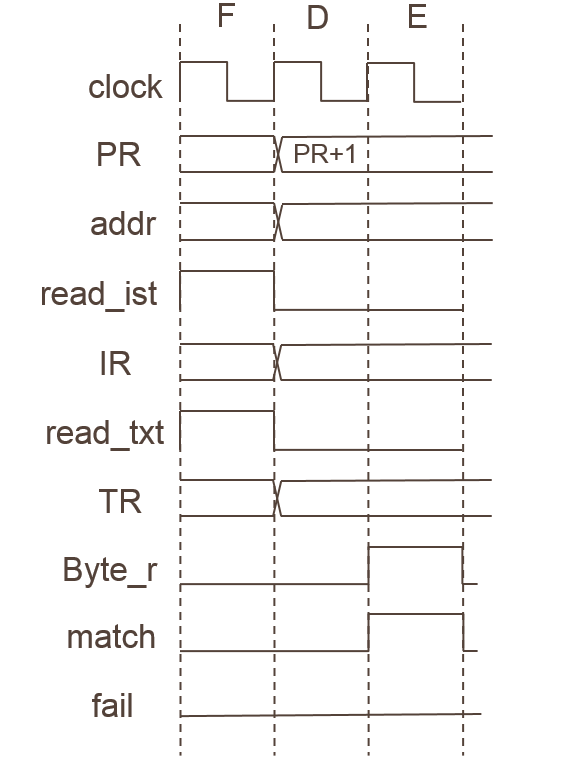
\includegraphics[width=30mm]{./fig/Byte}}
      \subfigure[Rbyte]{
        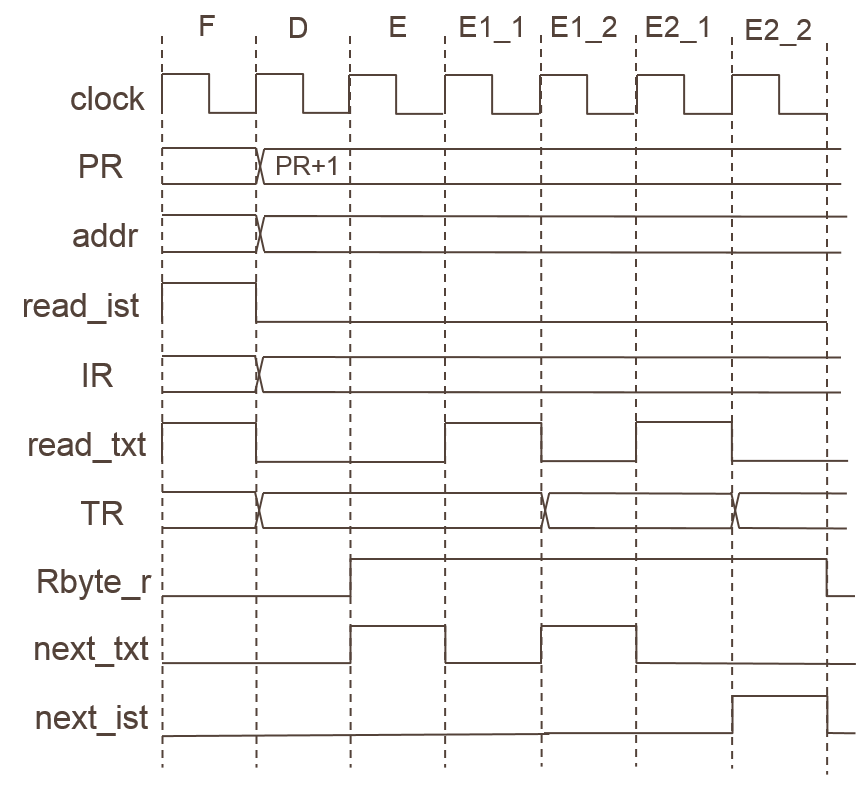
\includegraphics[width=45mm]{./fig/Rbyte}}
       \caption{Byte命令及びRbyte命令実行のタイムチャート }
 %       \label{Ist_list}
    %\end{center}
\end{figure}

Byte命令は、IRを持っている1文字のデータとTRの文字データを比較するのに対して、Set命令はTRの文字が複数の文字の中のどれかと一致するかを評価する命令である。Set命令を実行するために、Setテーブルを使う。Setテーブルは複数の256ビット列からなる。256ビット列に、ASCII表のn番目の文字とマッチさせるなら、nビット目を'1'にし、マッチさせないなら、'0'にする。Setテーブルは命令のバイトコードと同時に生成されている。このようにして、与えられた文字をSetテーブルに照らし合わせて、対応したビットの値は'1'であればマッチ成功、'0'であればマッチ失敗となる。\\

\subsubsection{特化命令}

特化命令Rbyteの実行では、F状態、D状態はByte命令と同様である。その様子は図5bに示すとおりである。Ex状態では、IRが持っている文字データとTRの文字データが一致した場合、next\_txt信号がハイレベルとなる。この場合、次のクロックサイクルの立ち上がりで文字読み込み信号のread\_txtがハイレベルとなり、FIFOから1文字を読み出す。次のクロックサイクルで、IRの持っている文字データと新たなTRの文字データを比較する。一致すれば、またFIFOから新たな文字を読み込まれる。IRの文字データとTRの文字データが一致しなくなるまで、この処理が繰り返される。一致しない場合、next\_ist信号がハイレベルとなり、次のクロックから新たな命令フェッチを実行する。

オプション命令(Obyte, Oset)も同様に実行されるが、文字消費信号を持っているところが違う。オプション命令はマッチ成功した場合、文字消費信号がハイレベルになり、文字を消費する。一方、マッチ失敗した場合、文字を消費しないが、Fail処理が起こらず、次の命令に進む。先読み命令(NByte, NSet)の実行もByte,Set命令の実行と類似するが、これらの命令では文字を消費しない。\\

\subsubsection{分岐命令}
%分岐命令には、Jump命令がある。Jump命令の実行は、デコードを行うクロックサイクルDecと、次に実行すべき命令のアドレスをプログラムレジスタ(PR)に転送するクロックサイクルからなる。各クロックサイクルで生成された制御信号を以下に示す。

分岐命令には、Jump命令がある。Jump命令実行のタイムチャートは図6に示すとおりである。E状態では、デコードした結果、Jump命令の実行のトリガーであるJump\_rがハイレベルになり、PRのトリガーであるPR\_lat信号もハイレベルになる。このとき、インクリメント信号のPR\_incはローレベルであるため、ジャンプ先のアドレスを持っているPC\_data\_inの値がPRに置き換える。次のクロックサイクルで、メモリアドレスレジスタaddrに少し遅れてPRの値が取り込まれる。また、次のクロックサイクルの立ち上がりで新たな命令フェッチが始まる。


\begin{figure}[h]
    \begin{center}
        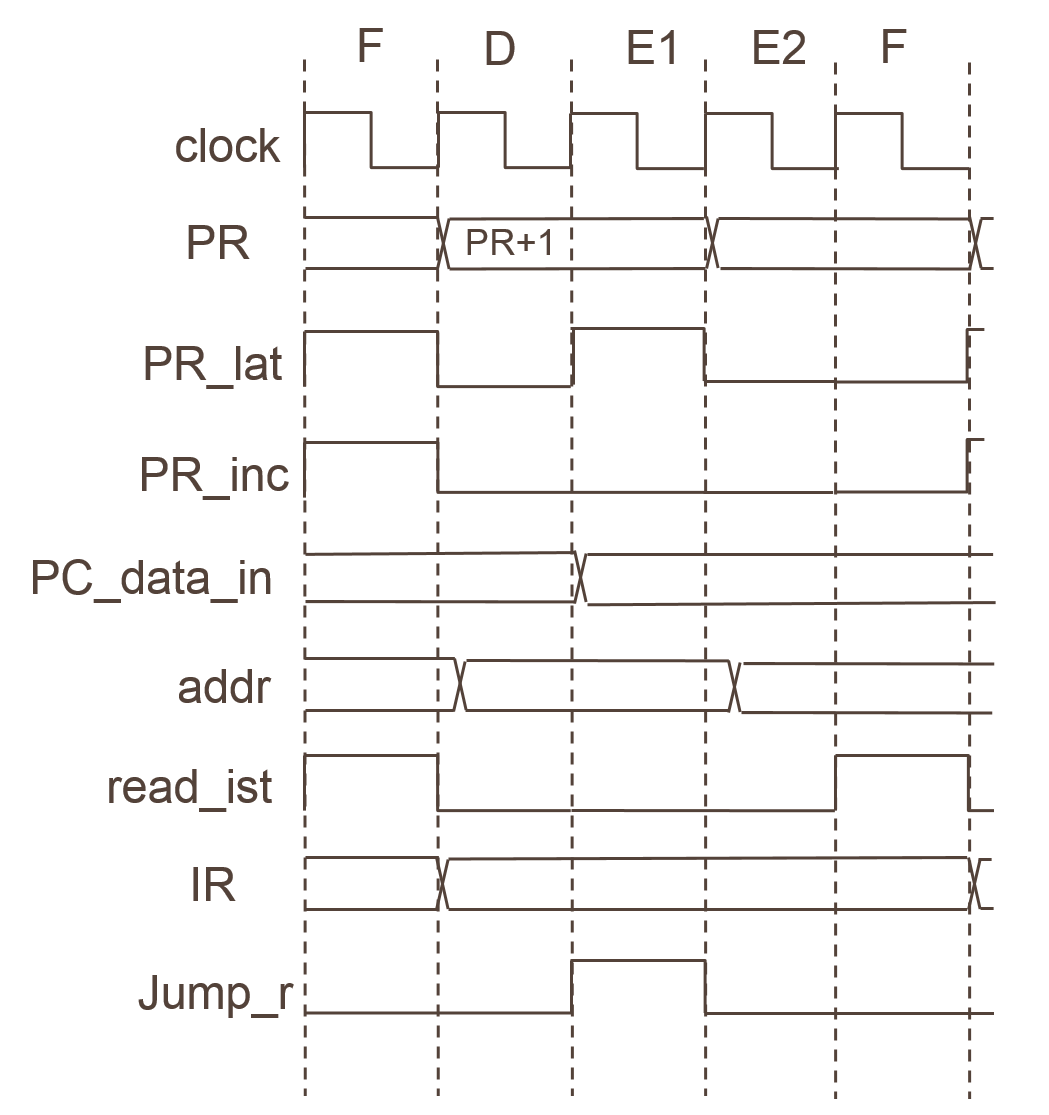
\includegraphics[width=50mm]{./fig/Jump}
       \caption{Jump命令実行のタイムチャート}
 %       \label{Ist_list}
    \end{center}
\end{figure}

\subsubsection{スタック操作命令}
スタック操作命令には、Call、Alt、Return、Succがある。

Non-Terminalを呼び出す命令がCall命令であり、それを呼び出したプログラムへ実行制御を返すのがReturn命令である。Call命令は、プログラムレジスタPRの値をReturnスタックにプッシュダウンして退避させ、Non-Terminalの先頭番地であるアドレスをPRに転送する。Call命令の実行はJump命令と類似しており、ただし新たなアドレスをPRに転送している同時に、Returnスタックにプッシュダウンを行う。

Return命令は、Call命令によってスタックに退避したNon-Terminalからの戻り番地をポップアップしてPRへ転送する。これによって、Non-Terminalを呼び出したプログラムへ実行制御が返される。Return命令実行のタイムチャートは図7に示すとおりである。

\begin{figure}[h]
    \begin{center}
        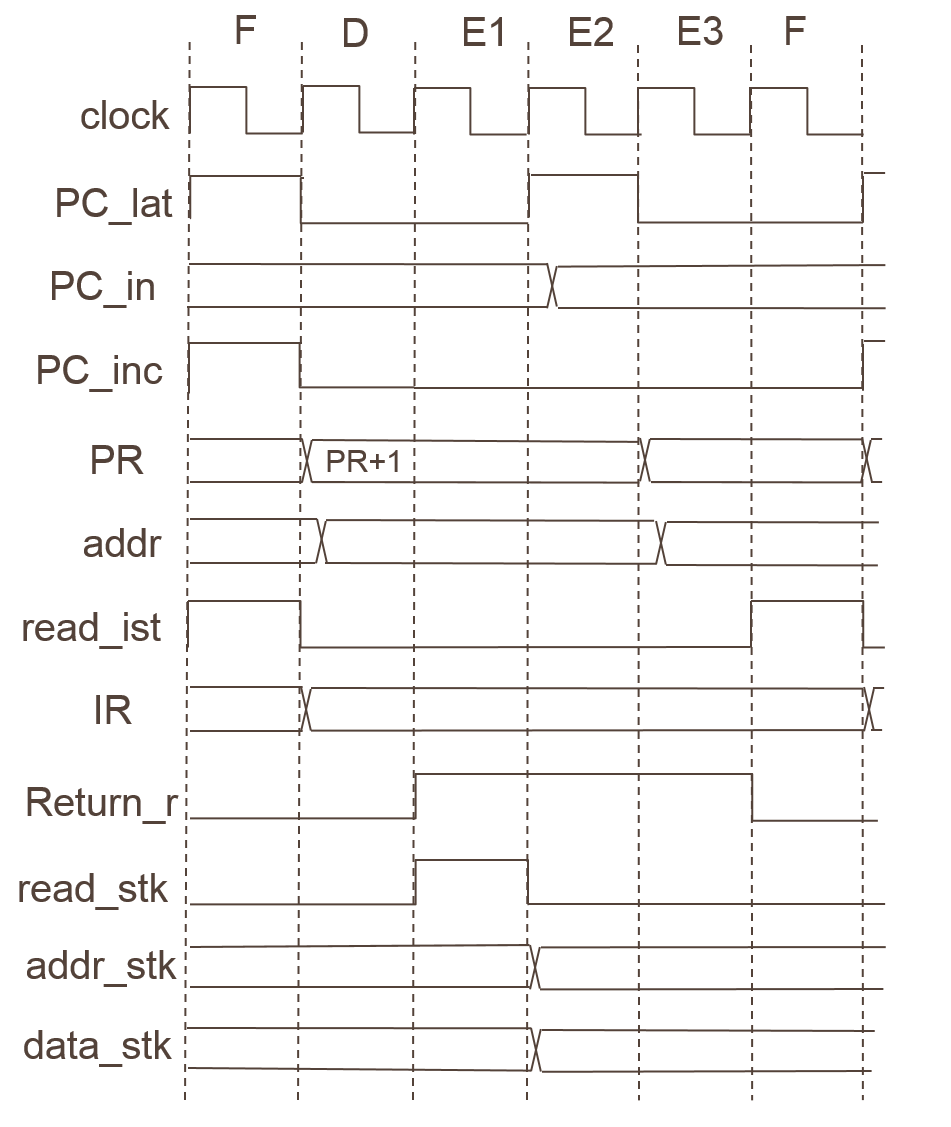
\includegraphics[width=50mm]{./fig/Return}
       \caption{Return命令実行のタイムチャート}
 %       \label{Ist_list}
    \end{center}
\end{figure}

E1状態のクロックサイクルの立ち上がりで、Return命令実行のトリガーであるReturn\_r信号がハイレベルになる。同クロックサイクルでReturnスタックの読み出し信号read\_stkがハイレベルになり、データをdata\_stkレジスタに転送される。次のクロックサイクルでPRの書き換えデータPC\_data\_inに少し遅れてdata\_stkのデータが取り込まれる。次のクロックサイクルの立ち上がりでPRの新たなアドレスが確立し、少し遅れて命令アドレスのaddrレジスタに転送される。このじて時点でReturnスタックからポップアップしたアドレスは次の命令を指すようになった。次に新たな命令フェッチが始まる。


%その実行ステップはデコードを行うクロックサイクルDecと、メモリスタックにデータをプッシュダウンするクロックサイクルEx、及びPRにポップアップされた命令アドレスへの転送を行うクロックサイクルからなる。同様に、スタックポインタのインクリメント及びスタックメモリアドレスの設定は既に実行済みである。各クロックサイクルで生成される制御信号は以下に示す(図)。

%Return命令はSucc命令と類似しているが、両者の違いは、Succ命令はFailスタックからポップアップした値を捨てるのに対して、Return命令はポップアップした値をPRへ転送する点である。

%Alt命令の実行ステップは、デコードを行うクロックサイクルDecと、メモリスタックにデータをプッシュダウンするクロックサイクルExからなる。スタックポインタのインクリメント及びスタックメモリアドレスの設定は、前回のスタックプッシュが終わり次第、すでに実行された。このため、Call命令は3つのクロックサイクルで実行が可能になる。クロックサイクルExが終ったら、新たな命令フェッチが実行される同時に、スタックポインタのインクリメントとスタックメモリアドレスの設定も実行される。各クロックサイクルで生成された制御信号を以下に示す。
%Succ命令も同様である。



%\subsubsection{割り込み}
一方、PEGでは、バックトラックがある。バックトラックは、選択がある場合、ある選択肢でマッチが失敗した場合、前の状態に戻り、別の選択肢を評価する仕組みである。選択がある場合、選択肢を評価する前に、バクトラックが起こるときの戻り先をFailスタックにプッシュダウンされる。これ操作を行うのはAlt命令である。

また、どこかでマッチが失敗した場合、バックトラックが起こる。このとき、Fail処理が行われ、FailスタックからポップアップされたアドレスをPRに転送され、次に実行される命令のアドレスになる。一方、無事にマッチできた場合、他の選択肢を評価する必要がなくなるため、Failスタックに保存したアドレスが除去される。この操作を行うのはSucc命令である。

Alt命令とSucc命令の動作はCall命令、Return命令と類似しているが、両者の違いはAlt命令とSucc命令がスタックを操作するだけで、PRにデータを転送しない点である。


%バックトラック処理では、Failスタックからポップアップするクロックサイクル、ポップアップされた値をPRへ転送するクロックサイクルからなる。バックトラック処理で生成される制御信号は以下に示す(図)。

\section{性能評価}

本研究では、Xilinx社のZynq xc7z010-1clg400cを搭載したZynq-7000評価ボードで実装した。また、VHDLによるRLT記述で行い、論理合成や配置配線、シミュレーションなどにはVivado Suite Design 2015.3を用いている。クロック周波数は125MHzである。

ホストとのインターフェースを除いたVirtual Machine本体の実装で用いたリソース使用量は表3に示すとおりである。

\begin{table}[h]
	\caption{リソース使用量}
	\centering
\begin{tabular}[t]{lccr}
	\hline\hline
	 リソース & 使用量 &  利用可能 & 使用率(\%) \\\hline
	 LUT & 323 & 17600 & 1.84 \\
	 FF & 196 & 35200 & 0.56 \\
	 ロジックセル & 565 & 28000 & 2.02 \\\hline
\end{tabular}
\end{table}
	 
現時点では、四則演算を表すなどの簡単なPEGに対して、正しく動作することが確認できた。表3に記載したリソースはPEGファイル及び文字列の複雑度に依存しない。ただし、BlockRAMの使用量はPEGファイル及び文字列の複雑度に依存する。

BlockRAMは、命令列領域、スタック領域、Setテーブルで使われている。命令列領域及びSetテーブルに用いられるメモリ量はPEGファイルに依存する。例えば、図1に示す四則演算を表すPEGの場合、4つのルールから34の命令が生成される。一つの命令は16bitであるため、命令列領域に34$\times$16bitが使われている。また、Setテーブルに3列が必要であり、つまり3$\times$216bitが使われている。命令列領域及びSetテーブルで使われるBlockRAMは合計で1192bitとなり、搭載された240KByte BlockRAMの0.062\%である。

一方、スタックに使われるメモリ量は文字列の長さや構造に依存するため、どの程度のメモリを確保すればよいかは今後の課題となる。



%実装環境\\

%C言語版との性能比較


\section{まとめ}

本稿では、解析表現文法(PEG)に特化したVirtual Machineについて述べた。必要最小限の回路だけ搭載し、またPEG演算子に特化した回路により、コンパクトかつ効率がよいマッチングマシンが実現できた。Virtual Machine本体が非常に小さいため、同じFPGAに複数のVirtual Machineを載せ、並列で動作させることによって、高いスループットのマッチングマシンが期待できる。

現時点では、四則演算を表すなどの簡単なPEGファイルに対して正しく動作できた。スタックに使われるメモリの見積、及びより複雑なデータ構造を処理できるように回路を拡張するのは今後の課題となる。

\bibliographystyle{ipsjunsrt.bst}
\bibliography{mybib}

\begin{thebibliography}{99}
\bibitem


\bibitem{okumura}
奥村晴彦:改訂第5版 \LaTeXe 美文書作成入門,
技術評論社(2010).

\bibitem{companion}
Goossens, M., Mittelbach, F. and Samarin, A.: {\it The LaTeX Companion},
Addison Wesley, Reading, Massachusetts (1993).

\bibitem{book1}
木下是雄:
理科系の作文技術,
中公新書(1981).

\bibitem{book2}
Strunk, W.J. and White, E.B.: {\it The Elements of Style, Forth Edition},
Longman (2000).

\bibitem{book3}
Blake, G. and Bly, R.W.: {\it The Elements of Technical Writing},
Longman (1993).

\bibitem{book4}
Higham, N.J.:
{\it Handbook of Writing for the Mathematical Sciences},
SIAM (1998).

\bibitem{webpage1}
情報処理学会論文誌ジャーナル編集委員会:
投稿者マニュアル(オンライン),
\urlj{http://www.ipsj.or.jp/journal/ submit/manual/j\_manual.html}%
\refdatej{2007-04-05}.

\bibitem{webpage2}
情報処理学会論文誌ジャーナル編集委員会:
べからず集(オンライン),
\urlj{http://www.ipsj.or.jp/journal/\\ manual/bekarazu.html}%
\refdatej{2011-09-15}.

\end{thebibliography}

\end{document}
